\begin{center}
  \section*{NetAppでつくる、OpenStackストレージ基盤 ~ストレージの選定で気をつけるべきポイント~}
\end{center}


\begin{flushright}
  \begin{itemize}
  \item   登壇者: 小林慶太,上田雅幸
  \item 資料: 
  \end{itemize}
\end{flushright}

\section*{概要}

YahooはOpenStackのストレージにNetApp社製品を採用し、Cinder volume boot環境とManilaサービスの提供をおこなっている。
NetApp社製品の採用に至った理由は、OpenStackコミュニティへの貢献度とネイティブAPIの提供の有無であった。
そして、クラスターとストレージを別々に構築し運用コストの削減を実現した。

\section*{詳細}

Yahooは、100以上のサービスを運用し、月間のページビューが752億になりデータ容量としては65PBにのぼる。
この大規模システムを1200000VMを構築し、VMを75000台の物理マシンで管理している。
膨大な物理マシンは、東西のDCに分けて管理しており、西日本に3DC、東日本に2DC保有している。

VMの管理にOpenStackを活用して5年になる。
OpenStackのストレージにNetApp製品を採用し、manilaサービスとCinder のvolume boot機能によるVMの管理を実現させた。
本発表は、NetApp製品の採用理由およびストレージの運用における課題とその解決についてである。\\

Yahooでは、OpenStackのクラスターが増加傾向にありそれに伴い設備投資および構築と運用のコストが増大していた。
この一因は、OpenStackのクラスター構築にストレージが必須であったためである。\\

そこで、ストレージのネットワークをL3ネットワークの専用のネットワーク構築し、拡張可能なストレージ設計をおこなった。
また、運用の利便性や堅牢性を担保するためにデータをポリシーごとに論理分割し、Manilaサービスを適用することとした。
compute ノードの性能向上のためにCinderのVolume Boot方式を採用した。\\

\href{https://wiki.openstack.org/wiki/Manila}{Manila} はCinderベース共有ファイルシステムを提供するOpenStackのコンポーネントである。
Manilaはファイル・ディレクトリ単位のアクセス制御を可能にし、管理下のデータをクラウド間で自由に移動させることができる機能を有している。\\

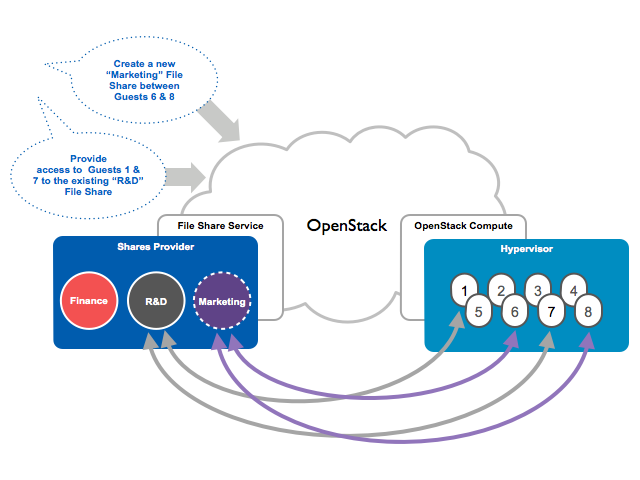
\includegraphics[width=10cm]{Manila_Concept.png}

データを主軸にシステムを設計することで、VMの集約率を高めることに成功した。
この構成の実現にあたりYahooは、NetAppの製品を採用した。
それは、NetAppがManilaへの貢献が多く知見を有していること、およびNetAppのストレージ製品がネイティブなAPIを有しておりManilaとの通信が独自でラップしやすくなっていたためである。
